% Plantilla creada por Francisco Javier Vázquez Tavares
% Esta platilla se creo para facilitar la creación de documentos para tareas.

\documentclass{tareaClass}

\title{ System ID: system-2025-05-15-230326-CL-0.5 }

\begin{document}
\lhead{ System ID: system-2025-05-15-230326-CL-0.5 }\rhead{ \today }

\maketitle

\section{General Parameters}

\begin{table}[ht!]
\centering
\begin{tabular}{|c|c|} 
\hline
Parameter & Value  \\ 
  \hline
    Packing fraction $\phi$ & 0.5 \\
    Crosslinker concentration & 0.5 \\
    Total central particles & 1500 \\
    Temperature & 0.05 \\
    Time step & 0.001 \\
    Box length (L) & 12.037717 \\
  \hline
\end{tabular}
\end{table}



\section{Assembly}

\begin{table}[ht!]
\centering
\begin{tabular}{|c|c|} 
\hline
Parameter & Value  \\ 
  \hline
    Damp value & 0.1 \\
    Time steps for heat up process & \num{500000} \\
    Time steps for isothermic process & \num{8000000} \\
    Fix saving frequency  & \num{10000} \\
    Stress saving frequency & \num{10000} \\
    Dump saving frquency  & \num{1000000} \\
  \hline
\end{tabular}
\end{table}

\begin{figure}[ht!]
\centering
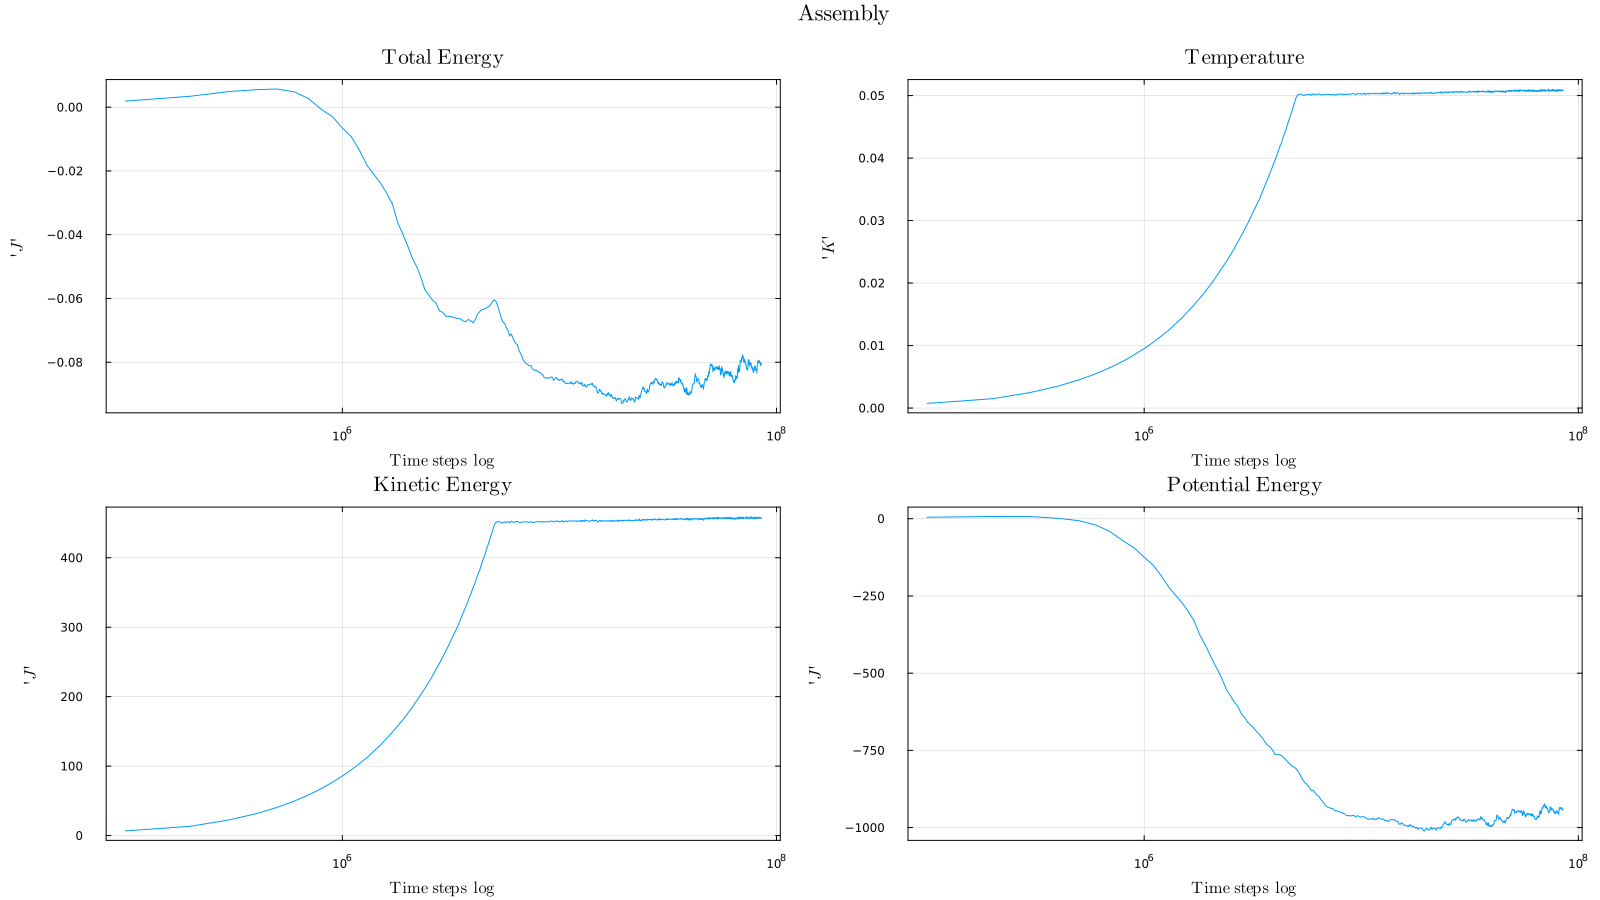
\includegraphics[width=\textwidth]{imgs/2025-05-15-230326-system_assembly.png}
\end{figure}

\newpage

\section{Shear}

\end{document}
